%!TEX root = 2017-icip-provenance-filtering.tex
\section{Experiments and Results}
\label{sec:experiments}
In this section, we present and discuss the experimental results we performed to validate the proposed method. We report the quality of the results in terms of Recall@k that measures the fraction of correct images at the top-$k$ retrieved results. The source code of all proposed methods are freely available\footnote{The source code is freely available on \url{https://gitlab.com/notredame-provenance/filtering}}.

\vspace*{0.1cm}
\noindent
\textbf{Datasets.} 
We adopt the Nimble Challenge 2016 (NC2016) and 2017 (NC2017) datasets, provided by the National Institute of Standards and Technology (NIST)~\cite{Nimble_2016}, which focus on forensics, provenance filtering and phylogeny tasks. These datasets comprise a query set containing different kinds of manipulated images (e.g., copy-move and compositions), and a gallery set containing the source images used to produce the queries. The datasets also comprise distractor images. The probe sets of NC2016 and NC2017 datasets contain $288$ and $16$ composite images, respectively. The gallery sets contain $874$ and $10446$ images, respectively. We also embed the datasets within one million images (distractors) provided by RankOne Inc.\footnote{\url{http://medifor.rankone.io/}}, as recommended by NIST for evaluating scalability. 

\vspace*{0.1cm}
\noindent
\textbf{Indexing Method.} We now analyze (see Table~\ref{tab:indexing_method}) different indexing approaches for NC2017 and NC2017+World1M in terms of memory footprint and efficiency (results for NC2016 are similar) considering an Intel(R) Xeon(R), CPU E5-2620 v3 @2.40GHz, 24 cores and 512GB of RAM. Although PQ is more efficient in terms of storage for a small scale, it does not scale for World1M. The clustering in HCAL prevented it from scaling for 1M images. More work involving approximate clustering and sampling would be necessary in this case. KD-Tree shows a good storage and efficiency tradeoff. 
%
\begin{figure}[t]
	\begin{center}
	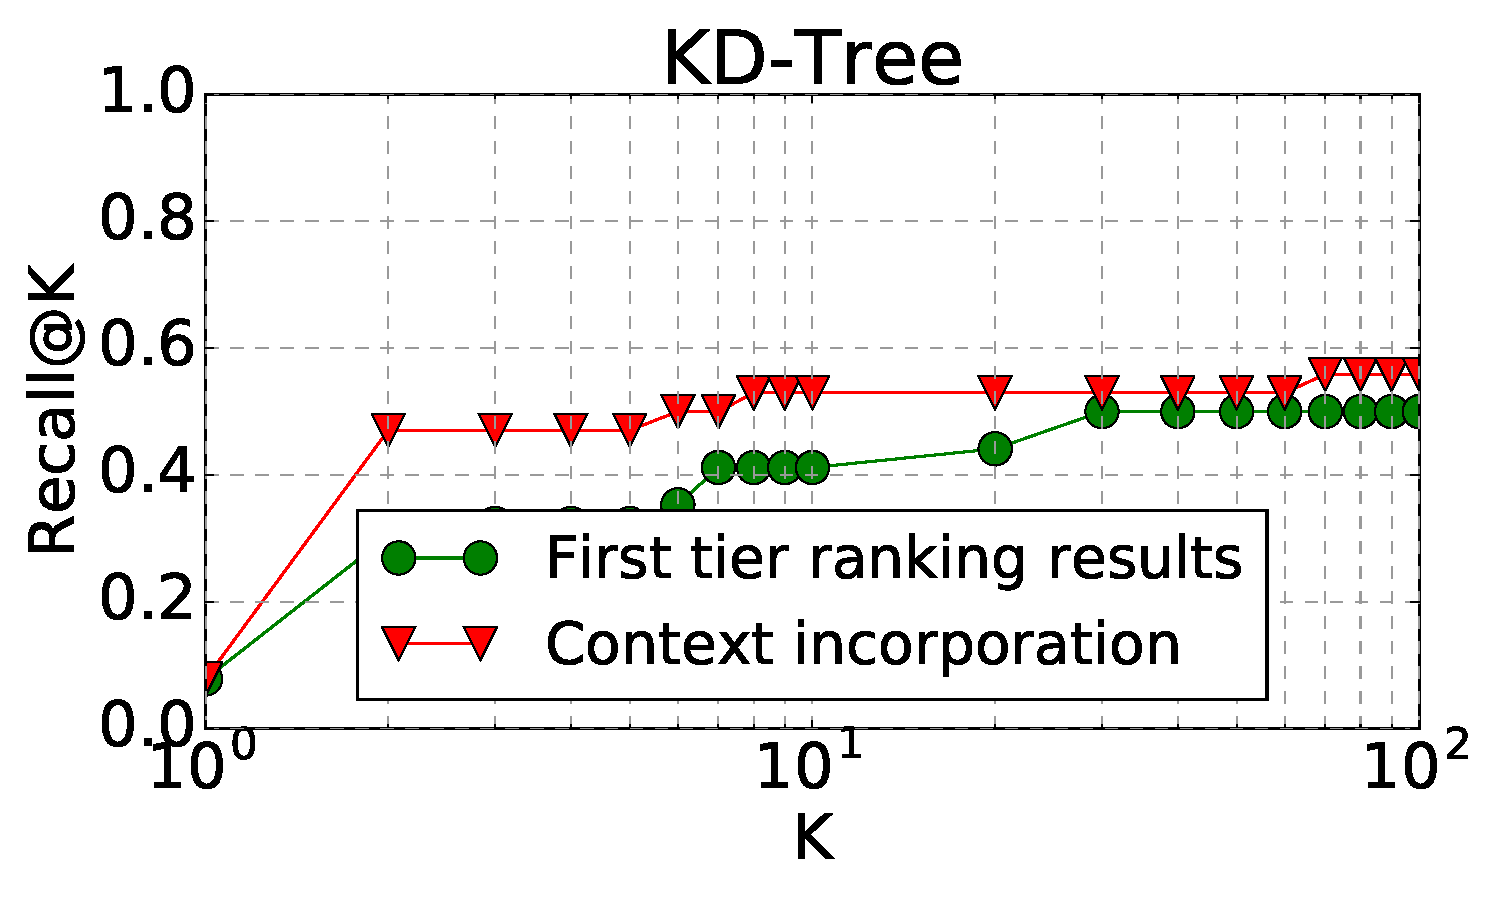
\includegraphics[width=0.48\linewidth]{nimble2017-alien-kdtree-recall_pr}
	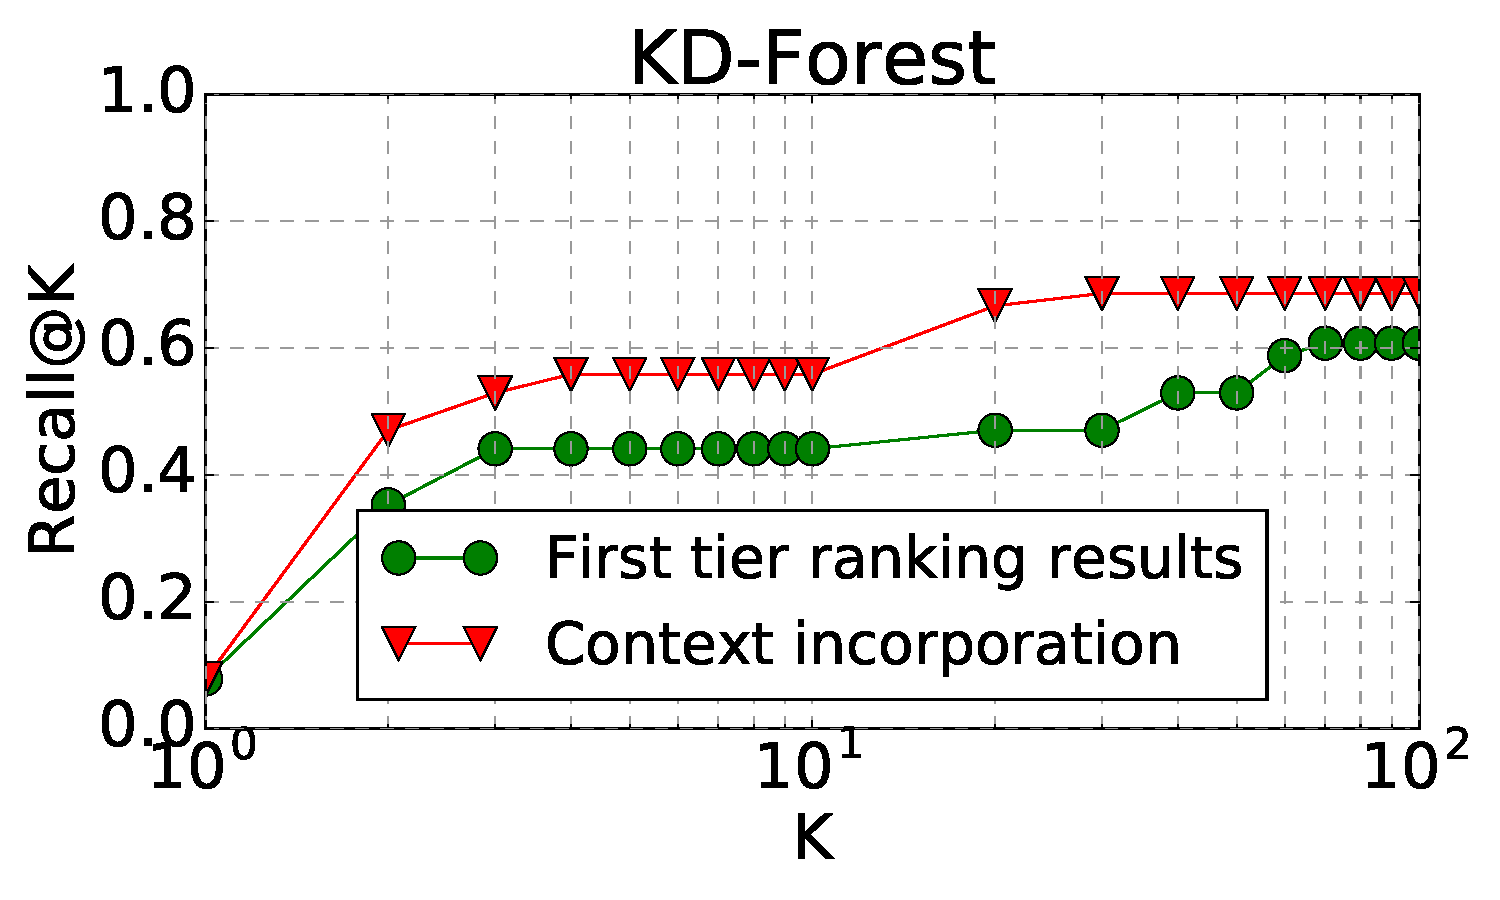
\includegraphics[width=0.48\linewidth]{nimble2017-alien-kdforest-recall_pr}
	\\
	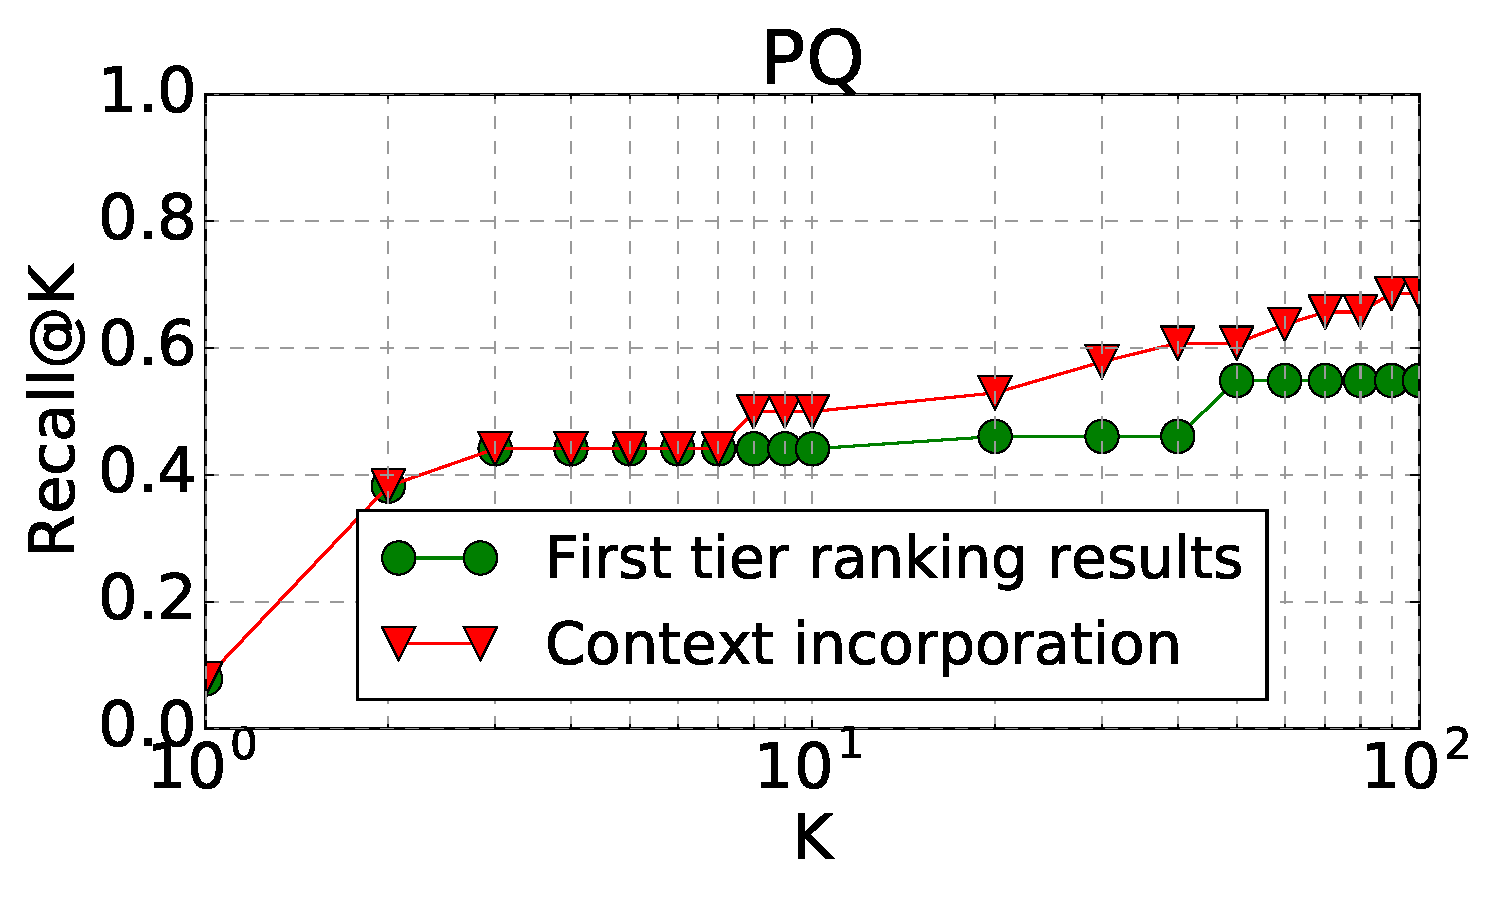
\includegraphics[width=0.48\linewidth]{nimble2017-alien-pq-recall_pr}
	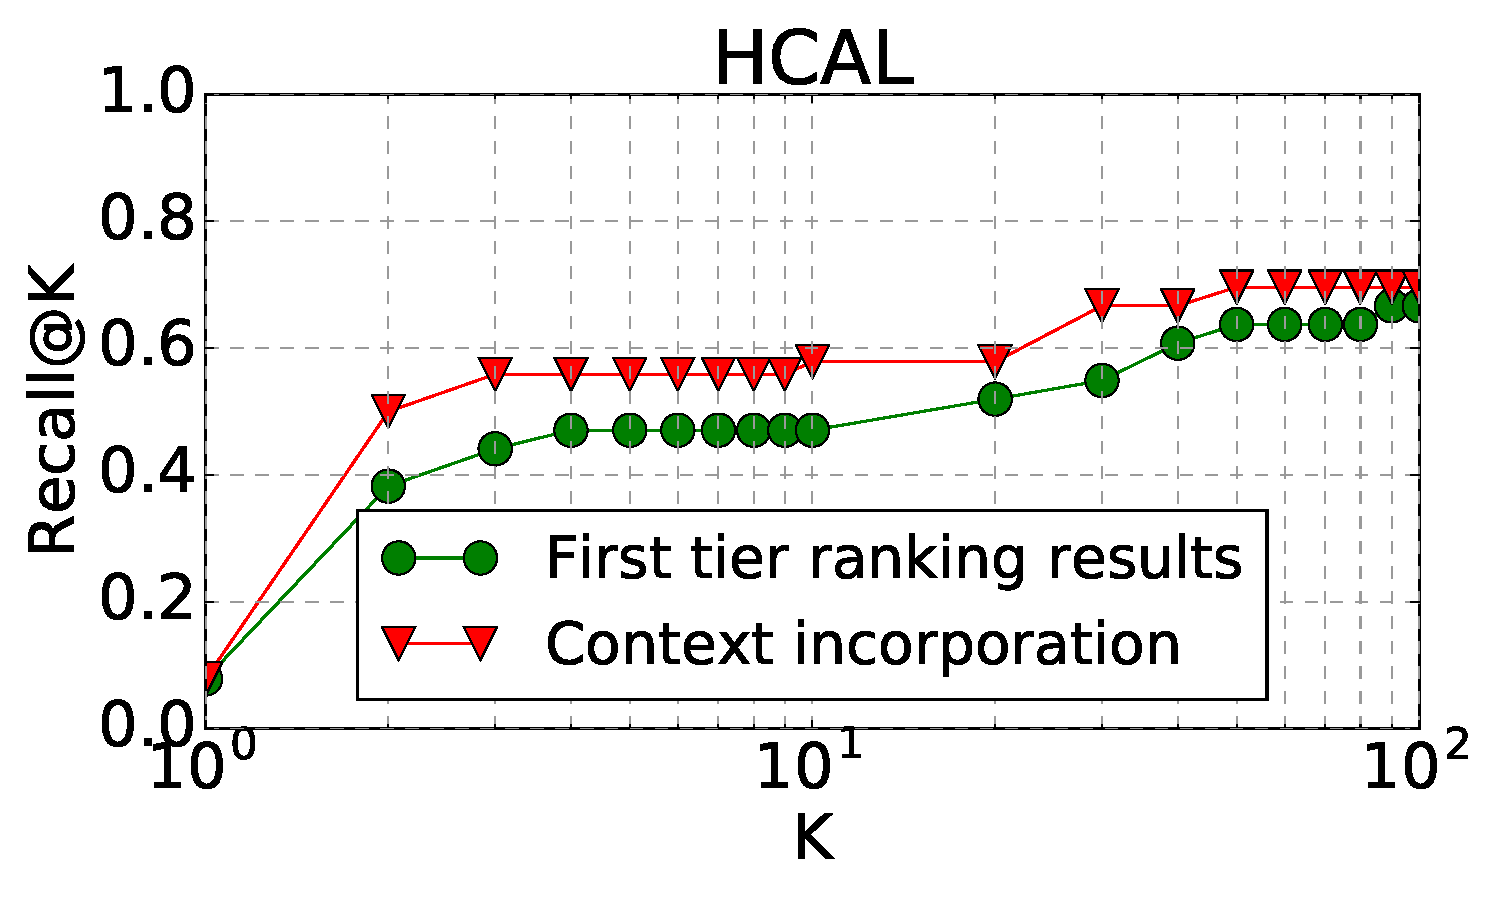
\includegraphics[width=0.48\linewidth]{nimble2017-alien-hcal-recall_pr}
	\caption{First- and second-tier results for the NC2017 dataset in terms of Recall@k. The context incorporation is important regardless of the  used indexing technique.\label{fig:indexing_compararison_2017}}	
	\end{center}	
\end{figure}

\begin{table}[t]
	\begin{center}
	\begin{footnotesize}	
	\setlength{\tabcolsep}{0.5em}
	\renewcommand{\arraystretch}{0.7}
	\caption{Runtime (in seconds) and memory usage (GB), per query, in the first tier, for different indexing techniques in the NC2017 and NC2017 + World1M datasets. KD-Forest comprises two trees. *~denotes the method did not scale.}
	\label{tab:indexing_method}
	\begin{tabular}{p{2.5cm}p{1.2cm}p{1.5cm}p{1.1cm}p{1.cm}}
		\topline
		\headcol \textbf{Method} & \textbf{KD-Tree} & \textbf{KD-Forest} & \textbf{PQ} & \textbf{HCAL} \\
		\midline
		\textbf{Runtime} & $0.69$ s& $0.72$ s& $13.96$ s& $0.85$ s\\
		\rowcol \textbf{Memory} & $1.48$ GB & $10.69$ GB & $0.02$ GB & $5.38$ GB \\
\hline
		\textbf{Runtime (World1M)} & $8.8$ s& $7.61$ s& $*$ & $*$ \\
		\rowcol \textbf{Memory (World1M)} & $34.99$ GB & $66.42$ GB & $*$  & $*$  \\
		\bottomlinec
	\end{tabular}
	\end{footnotesize}	
	\end{center}	
\end{table}

\vspace*{0.1cm}
\noindent
\textbf{Context Incorporation and Ranking Aggregation.} In this section, we evaluate the proposed approach to improve ranking results for donor images. 
Fig.~\ref{fig:indexing_compararison_2017} shows the performance results in terms of recall at the top-$k$ retrieved images, considering the retrieval of donor images in the first and second tiers of the proposed method. Although not shown here, the performance for retrieving the host image is always above 95\% as it shares much content with $q$. The challenge in provenance filtering is in retrieving the donors.

\vspace*{0.1cm}
\noindent
\textbf{Large-scale Image Retrieval.} We now evaluate the proposed approach, considering a more challenging scenario, in which we embed the NC2016 and NC2017 datasets into one million images, hereinafter referred to as World1M dataset. The World1M dataset contains several images that are semantically similar to the images that compose both datasets. Table~\ref{tab:large_scale_experiments} shows the obtained results in this experiment. There is a gain of about $7\%$ when retrieving donors for  NC2016 when we compare the obtained results in the first and second tiers. The results for NC2017 are slightly lower given that the composite images in this dataset are more difficult, more photorealistic and smaller with respect to the whole image, which also impacts the context incorporation, second tier (first- and second-tier results remain equal for this case). A future work consists of improving the context incorporation mask to better capture small donors such as those present in NC2017. 

% NC2016+1M: 1st tier -> Host: 99.65% - 2nd tier: 100.00%
% NC2017+1M: 1st tier: 88.24% - 2nd tier: 88.24%

\begin{table}[t]
	\begin{center}
	\begin{footnotesize}
	\setlength{\tabcolsep}{0.4em} % for the horizontal padding
	\renewcommand{\arraystretch}{0.7}% for the vertical padding	
	\caption{Performance results for NC2016 and NC2017 datasets embedded in one million images and KD-Forest (2 trees). Bold highlights improvements in the second tier.\label{tab:wds}}
	\label{tab:large_scale_experiments}
	\begin{tabular}{p{2.8cm}ccc}
		\topline
		\headcol \multicolumn{1}{c}{\textbf{Dataset}}		& \textbf{Type} & \textbf{Tier} & \textbf{Recall@10} \\
		\midline
		
		& 							& 1st 	& $99.65\%$ \\
		\multirow{-2}{*}{\textbf{NC2016 + World1M}}			& \multirow{-2}{*}{{Host}} 	& 2nd 	& $\textbf{100.00}\%$ \\
		\cline{2-4}\rowcol									&  							& 1st 	& $63.00\%$ \\
		\rowcol\multirow{-2}{*}{\textbf{NC2016 + World1M}}	& \multirow{-2}{*}{{Donor}}	& 2nd 	& $\textbf{67.71}\%$ \\
		\hline

		& 							& 1st 	& $88.24\%$ \\
		\multirow{-2}{*}{\textbf{NC2017 + World1M}}			& \multirow{-2}{*}{{Host}} 	& 2nd 	& $88.24\%$ \\
		\cline{2-4}\rowcol									&  							& 1st 	& $25.49\%$ \\
		\rowcol\multirow{-2}{*}{\textbf{NC2017 + World1M}}	& \multirow{-2}{*}{{Donor}}	& 2nd 	& $25.49\%$ \\
		\bottomlinec
	\end{tabular}
	\end{footnotesize}
	\end{center}	
\end{table}


\vspace*{0.1cm}
\noindent
\textbf{Qualitative Analysis.} Fig.~\ref{fig:qualitative} shows the results of two queries for KD-Forests with two trees in the first and second tiers. 

\begin{figure}[t]
	\begin{center}
	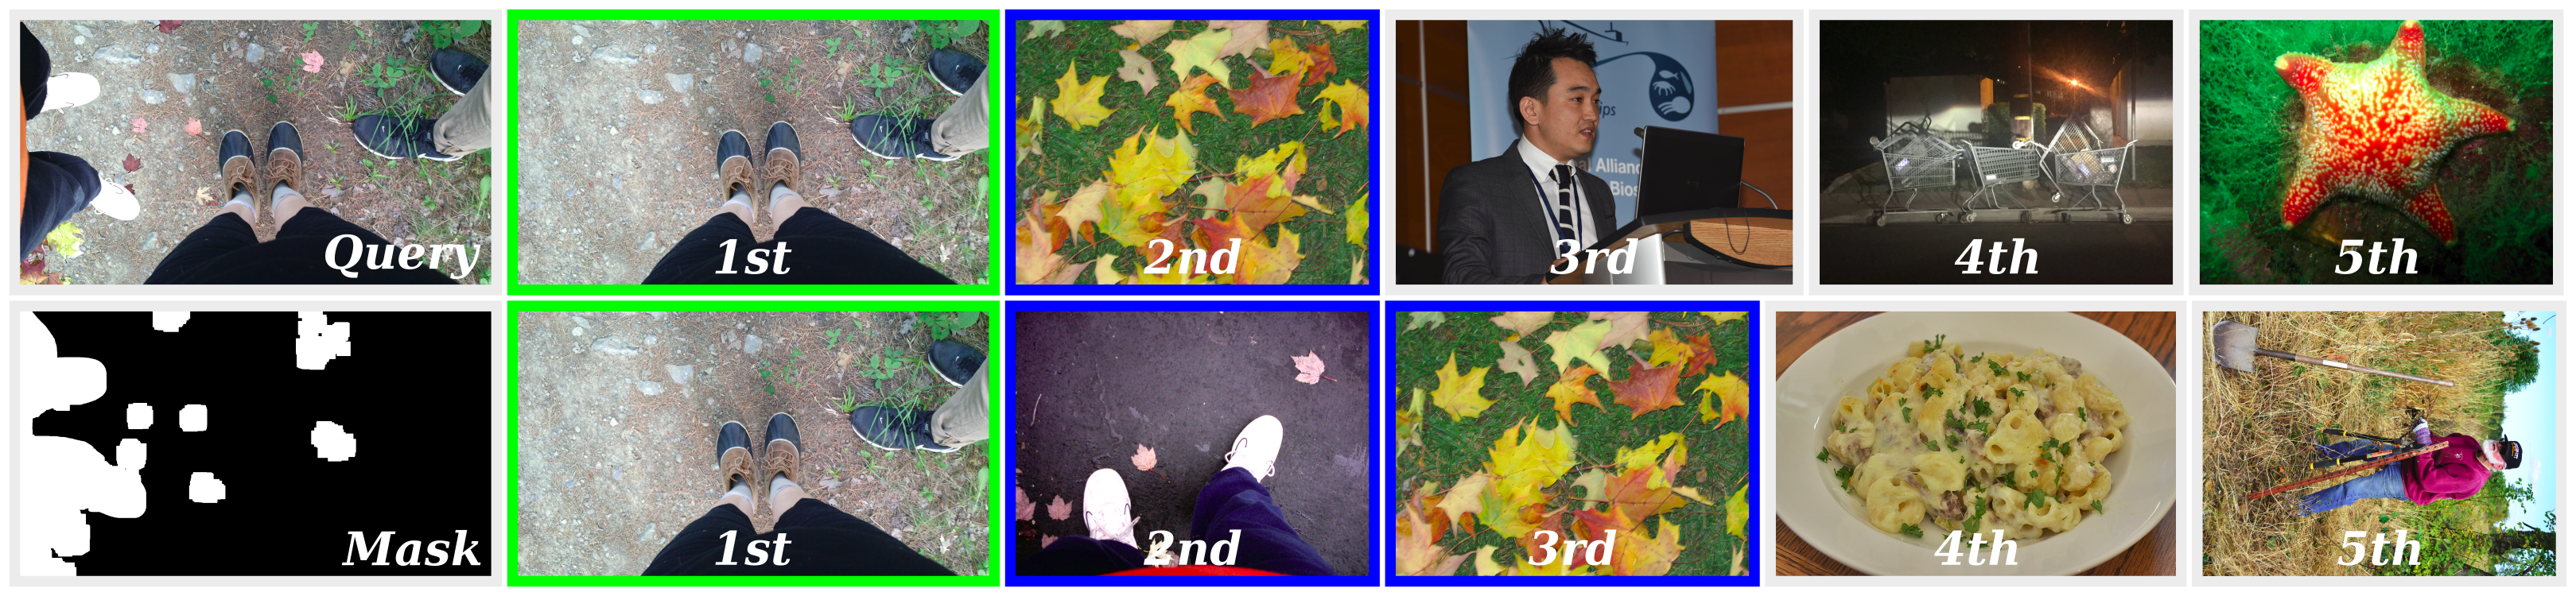
\includegraphics[width=0.8\linewidth]{qualitative_results_example_1.png}
	\vspace{0.3cm}
	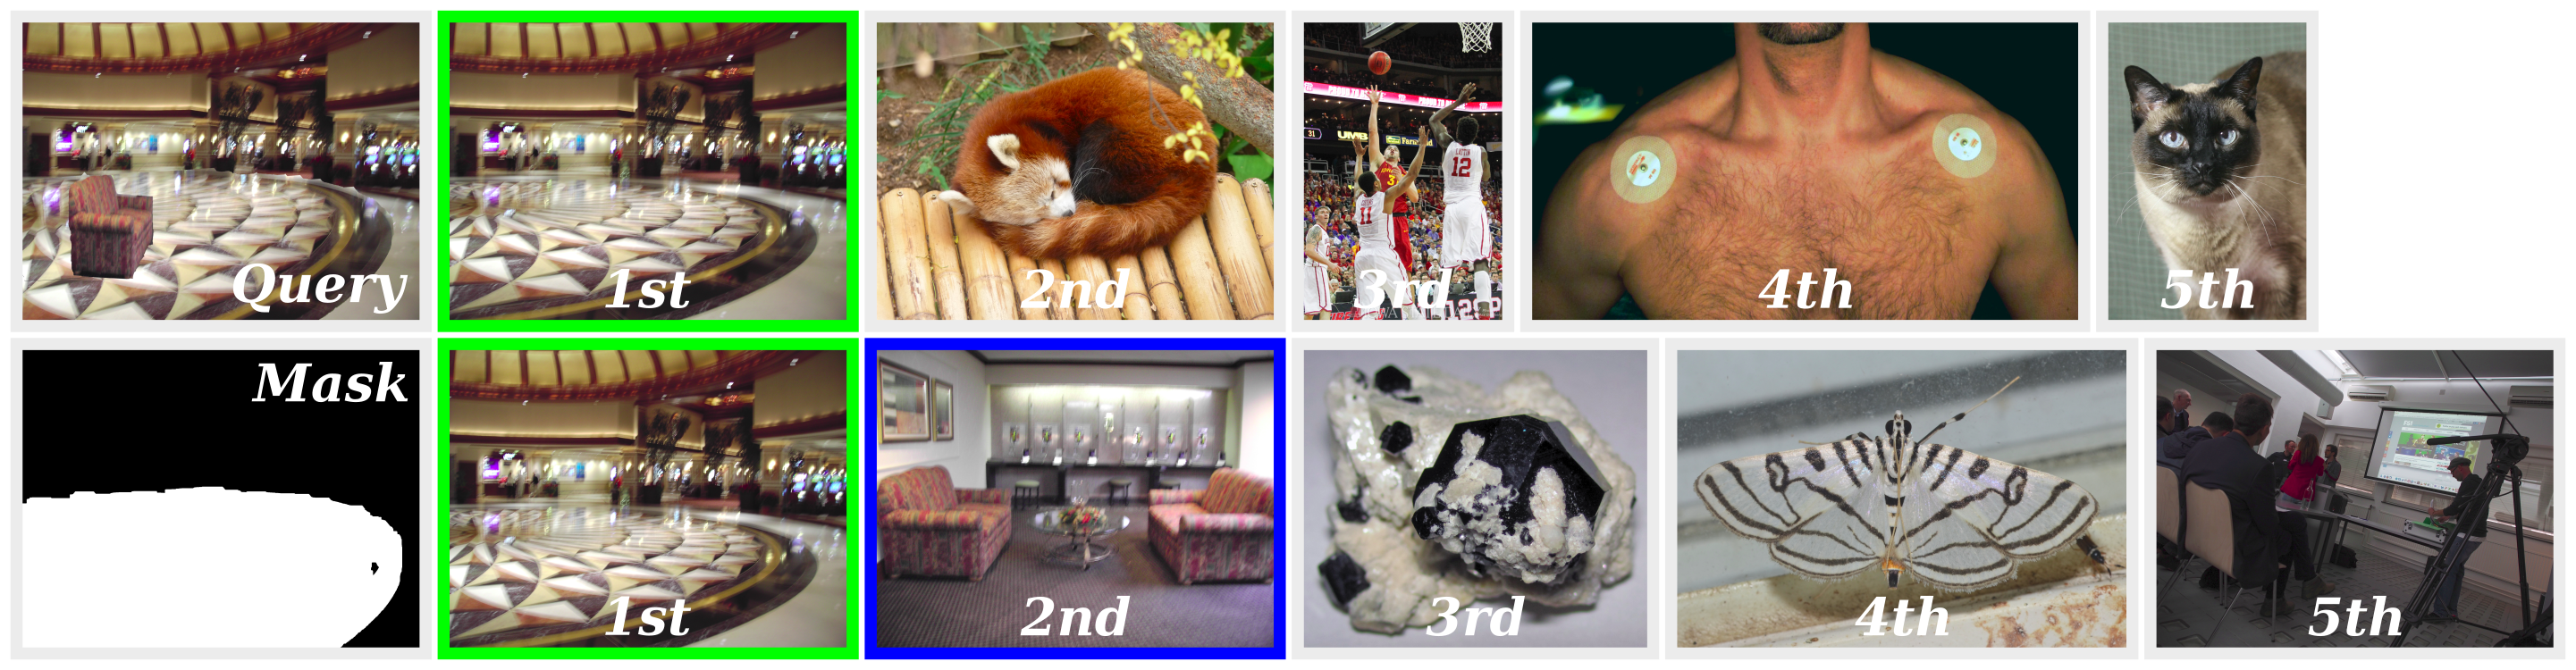
\includegraphics[width=0.8\linewidth]{qualitative_results_example_3.png}
	\caption{Queries and results for KD-Forest + 2 trees. The first and third rows refer to the first tier results while the second and fourth refer to the second tier. The green border denotes the matched host while the blue ones denote donors. The search in the second tier allows the retrieval of donors that were not present in the first tier.\label{fig:qualitative}}	
	\end{center}	
\end{figure}
